\section{Introduction}

To realize the vision of the Semantic Web, the conformance of existing data to the RDF model is a necessary condition. Yet, it is a fact that most of the data available on the Web do not satisfy the latter requirement. A number of tools have been developed to facilitate the transition to RDF. Much of them are founded on well-defined mapping languages (R2RML~\cite{R2RML_W3C:12}, RML~\cite{dimou2014rml}, SPARQL-Generate~\cite{lefranccois2016flexible}, etc.). Using mapping languages directly is complex. This is because they have a steep learning curve and require knowing the syntax and semantics of the languages in addition to the Semantic Web stack and ontologies that can be used. 

Besides mapping languages, there are automatic and semi-automatic RDFizers. We ignore automatic RDFizers (e.g. Direct Mapping~\cite{Direct_Mapping_W3C:12}, Docker2RDF~\cite{ayed2017docker2rdf}, etc.) as their transformation cannot be customized or they are restricted for specific domain models. The minor category of works (RMLEditor~\cite{heyvaert2016rmleditor}, OpenRefine~\cite{verborgh2013using}, etc.) around semi-automatic RDFizers is our main interest. We focus on this category due to their ability in aiding human experts by automating complex tasks without hindering flexibility by incorporating them for decision making and validation. The main problem with the latter tools is that they mostly only provide a graphical interface with some facilities for searching through ontologies. However, they depend much on human experts with respect to knowledge about ontologies and data modeling using them.

In this work, our aim is to provide an approach to further facilitate semi-automatic RDFizers by automatically generating initial mappings that may then be customized by human experts. The originality of our contribution is that it automatically generates several holistic mappings and try best to provide an exhaustive description for a given type of instances. Our approach is not an alternative but complementary to existing tools. In the rest of this paper, we describe our approach and its implementation in \secref{approach} and \secref{implementation} respectively. Finally, we demonstrate our implementation using real datasets from open data portal. %Finally, we describe \secref{futureWork} that are we are currently working on.   



\section{Our Approach}\label{sec:approach}
Our approach to generate initial mappings consists of four main steps as shown in \figref{overviewApproach}. For illustration purposes, we consider a parking dataset\footnote{\url{http://data.metropolegrenoble.fr/ckan/dataset/parkings-de-grenoble/resource/a6919f90-4c38-4ee0-a4ec-403db77f5a4b}, last accessed on 7 December 2019} from Grenoble open data portal\footnote{\url{http://data.metropolegrenoble.fr/}, last accessed on 7 December 2019}. \figref{sampleRawData} is part of a preview of that dataset taken directly from the data portal.

\begin{figure}[h]
	\centering
	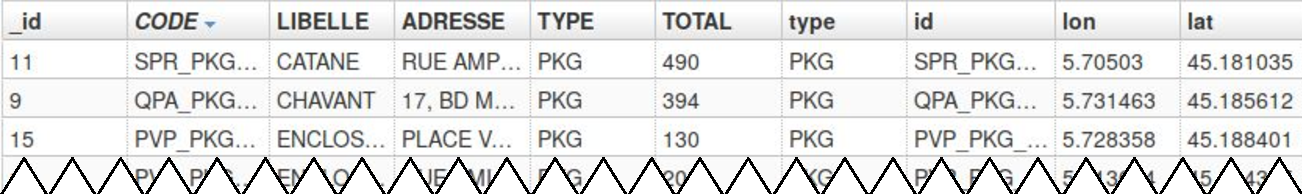
\includegraphics[scale=0.45]{images/sampleRawData.pdf}
	\caption{Parking data from Grenoble Open Data Portal}
	\label{fig:sampleRawData}
\end{figure}

Moreover, our approach uses an \kword{Ontology repository}. Suppose that it contains the vocabularies MobiVoc\footnote{\url{https://www.mobivoc.org/}, last accessed 10 February 2020}, Schema.org\footnote{\url{https://schema.org/}, last accessed 10 February 2020}, WGS84\footnote{\url{https://www.w3.org/2003/01/geo/}, last accessed 10 February 2020} and Dublin Core Metadata Terms\footnote{\url{https://www.dublincore.org/specifications/dublin-core/dcmi-terms/}, last accessed 10 February 2020}. 

\begin{figure}
	\centering
	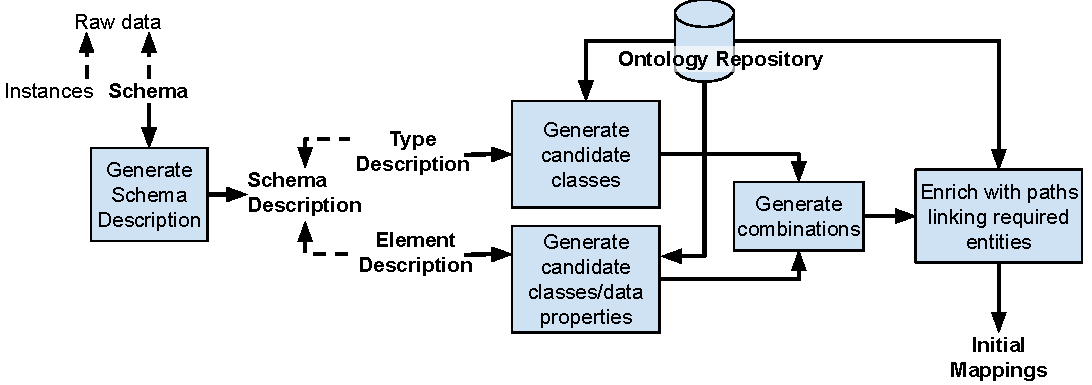
\includegraphics[scale=0.55]{images/GeneralApproachPaper1.pdf}
	\caption{Mappings Generation Process}
	\label{fig:overviewApproach}
\end{figure}

In our approach, to capture the background knowledge about the schema used in the raw data, firstly, we generate a \kword{Schema description} consisting of a \kword{Type description} and a \kword{Elements description}. \kword{Type Description} characterizes using keywords the type of objects described by the schema. \kword{Elements description} characterizes using keywords the schema elements (e.g. \kword{lon} in \figref{sampleRawData}).   


Secondly, using an \kword{Ontology repository}, and the \kword{Type description} and the \kword{Elements description}, a set of candidate classes are generated for typing objects and a set of candidate data properties or classes are generated for modeling the schema element. \nath{donner des détails : Existing simple matching approaches such as those presented in xx can be used at this step. et après mettre dans implem qq mots sur celles qu'on utilise nous}

\tabref{overviewElementMappings} shows a schema description for the schema of \figref{sampleRawData} and generated ontology entities for its elements. For example, the objects' type in \figref{sampleRawData} can be described by the keyword `parking facility'. Using the latter description, the classes \kword{mv:ParkingFacility} and \kword{sc:Park} are generated to type the objects. Similarly, the schema element \kword{TOTAL} is described using the keywords `capacity' and `total' using which the class \kword{mv:Capacity} and data property \kword{sc:totalTime} are candidate classes generated to model it. The candidate proposal \kword{sc:totalTime} is not appropriate to model \kword{TOTAL} as its semantics is not compatible with the latter. To determine the appropriateness of an entity, we also generated a confidence. For simplicity sake, we omit this information from \tabref{overviewElementMappings}.




\begin{comment}
For example, suppose the \kword{Type Description} include the keyword `parking facility' to describe the objects' type in \figref{sampleRawData}. This description is used to generate candidate classes that include \kword{mv:ParkingFacility} and \kword{sc:Park}.

Similarly, suppose the \kword{Elements Description} for the schema element \kword{TOTAL} and \kword{lon} in \figref{sampleRawData} include the keywords `capacity' and `longitude' respectively.

Using these descriptions, the candidate classes and data property generated for \kword{TOTAL} include \kword{mv:Capacity} and \kword{sc:totalTime} respectively.

Similarly, the candidate data property generated for \kword{lon} is \kword{wgs84:long}.
\end{comment}


%\vspace{-0.5cm}
\begin{table}[]
	\centering
	\scalebox{0.7}{
		\begin{tabular}{|l|l|l|l|l|}
			\hline
			\multicolumn{3}{|c|}{\textbf{Schema Description}}                                                                         & \multicolumn{2}{c|}{\textbf{Generated Entities}}                                                 \\ \hline
			&          & \textbf{Keyword}   & \textbf{Classes}                                                      & \textbf{Data Properties} \\ \hline
			\textbf{\begin{tabular}[c]{@{}l@{}}Type \\ Description\end{tabular}}                      &          & `parking facility' & \begin{tabular}[c]{@{}l@{}}\kword{mv:ParkingFacility},\\ \kword{sc:Park}\end{tabular} &                          \\ \hline
			\multirow{6}{*}{\textbf{\begin{tabular}[c]{@{}l@{}}Elements \\ Description\end{tabular}}} & \kword{id}       & `identifier'       &                                                                       & \kword{dc:identifier}            \\ \cline{2-5} 
			& \kword{LIBELLE}  & `description'      &                                                                       & \kword{sc:description}           \\ \cline{2-5} 
			& \kword{TOTAL}    & `capacity',`total' & \kword{mv:Capacity}                                                           & \kword{sc:totalTime}             \\ \cline{2-5} 
			& \kword{lat}      & `latitude'         &                                                                       & \kword{wgs84:lat}                \\ \cline{2-5} 
			& \kword{lon}      & `longitude'        &                                                                       & \kword{wgs84:long}               \\ \cline{2-5} 
			& \kword{ADDRESSE} & `address'          &                                                                       & \kword{sc:address}               \\ \hline
	\end{tabular}}
	\caption{Candidate entities for typing and schema elements}
	\label{tab:overviewElementMappings}
\end{table}
%\vspace{-1cm}


Thirdly, possible combinations are generated\nath{using a cartesian product}. A combination consists of a candidate class for typing, that we refer as the \emph{type class}, and a candidate data property or class for each schema element if it was generated in the previous step. \tabref{overviewCombinationsElements} shows all combinations generated from the candidate entities in \tabref{overviewElementMappings}. As we can see, in each combination, there is one candidate entity for the type class and schema elements.

%\vspace{-0.5cm}
\begin{table}[]
	\centering
	\scalebox{0.7}{
		\begin{tabular}{|l|l|l|l|l|l|l|l|}
			\hline
			& \textbf{Type Class} & \textbf{id}   & \textbf{LIBELLE} & \textbf{TOTAL} & \textbf{lat} & \textbf{lon} & \textbf{ADDRESSE} \\ \hline
			1. & \kword{mv:ParkingFacility}  & \kword{dc:identifier} & \kword{sc:description}   & \kword{mv:Capacity}    & \kword{wgs84:lat}    & \kword{wgs84:lon}    & \kword{sc:address}        \\ \hline
			2. & \kword{mv:ParkingFacility}  & \kword{dc:identifier} & \kword{sc:description}   & \kword{sc:totalTime}   & \kword{wgs84:lat}    & \kword{wgs84:lon}    & \kword{sc:address}        \\ \hline
			3. & \kword{sc:Park}             & \kword{dc:identifier} & \kword{sc:description}   & \kword{mv:Capacity}    & \kword{wgs84:lat}    & \kword{wgs84:lon}    & \kword{sc:address}        \\ \hline
			4. & \kword{sc:Park}             & \kword{dc:identifier} & \kword{sc:description}   & \kword{sc:totalTime}   & \kword{wgs84:lat}    & \kword{wgs84:lon}    & \kword{sc:address}        \\ \hline
	\end{tabular}}
	\caption{Combinations of generated entities for type class and schema elements}
	\label{tab:overviewCombinationsElements}
\end{table}
%\vspace{-1cm}

Finally, we enrich each combination with the required ontology entities to instantiate them for every object in the raw data.\nath{pas clair : we enrich each combination with the required ontology entities to describe  the Type Classe with the identified class or dataproperty mapped to an element description} For example, \figref{combinationNoPath} shows the first combination from \tabref{overviewCombinationsElements} and the required paths, illustrated as dotted lines, that will be generated at this step. It is possible that more than one paths or no paths exist between some entities. \nath{To identify such paths we ...}A combination and the required paths makes up one initial mapping. To choose an initial mapping and further customize it by choosing and validating the paths, a user interface is provided.

%\figref{sampleOntologyRawData} is a possible result with some of the paths generated. 



%For example, in the third combination from \tabref{overviewCombinationsElements}, there may be no path between the type class \kword{sc:Park} and the candidate class of \kword{TOTAL} that is \kword{mv:Capacity} . In this case, a human expert may chose to ignore this mapping     

%\vspace{-0.5cm}
\begin{figure}
	\centering
	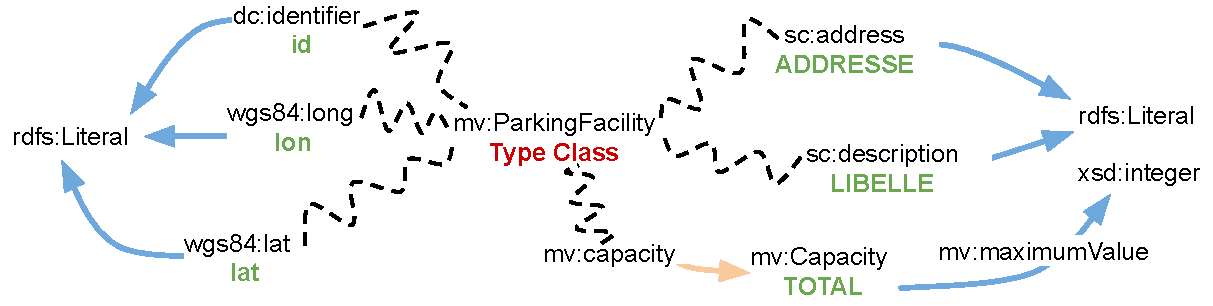
\includegraphics[scale=0.4]{images/combinationNoPath.pdf}
	\caption{Final mapping for first combination without generated paths}
	\label{fig:combinationNoPath}
\end{figure}
%\vspace{-1cm}

\section{Implementation}\label{sec:implementation}
An overview of our implementation is shown in \figref{OverviewImplementation}. Core to this implementation is the \kword{RDFizer} that generate initial mappings using the approach described in the previous section. To facilitate human intervention,
we provide a graphical \kword{User Interface}. Using the interface, users can upload the raw data in the CSV format and may enrich it with keywords to generate the \kword{Schema description}. The \kword{User Interface} interacts with the \kword{RDFizer} via a \kword{Web Service}. Eventually, on obtaining the initial mappings, one of them is chosen and, refined and validated by the human expert and sent to the web service together with the raw data for transformation to RDF.

\begin{figure}[h]
	\centering
	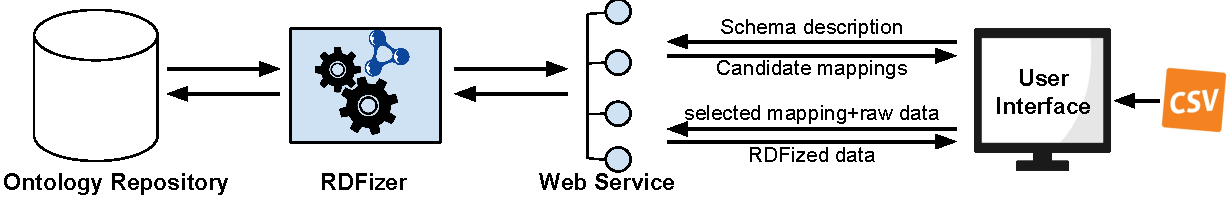
\includegraphics[scale=0.55]{images/OverviewImplementation.pdf}
	\caption{Overview of Implementation}
	\label{fig:OverviewImplementation}
\end{figure}

The user interface is a web application implemented using the JavaScript library \emph{React}\footnote{\url{https://reactjs.org/}}. The video shows the use the interface to generate mappings for the CSV parking dataset in \secref{approach}. As it can be seen, the user interface (\figref{screenshotInterface}) has three main parts. The top left part is focused on the raw data that is imported using the \kword{import CSV} menu item. On clicking on a column, keywords can be entered. The bottom left part shows the initial mappings and on selecting one of them, its corresponding description graph is rendered on the right part. The human expert can interact with different part of the latter graph and select and validate the paths. 

%For each possible mapping in the bottom right part, different pieces of information are provided namely: score, type class, number of classes/data properties and finally number of (un)mapped columns. Two main refinements are possible for each possible mapping. Firstly, data properties can be specified in class mappings. Secondly, ontology entities can be changed and paths can be re-generated for any schema element. This gives the user full flexibility to change and adapt a particular possible mapping.     


\begin{comment}
	\begin{figure}[h]
	\centering
	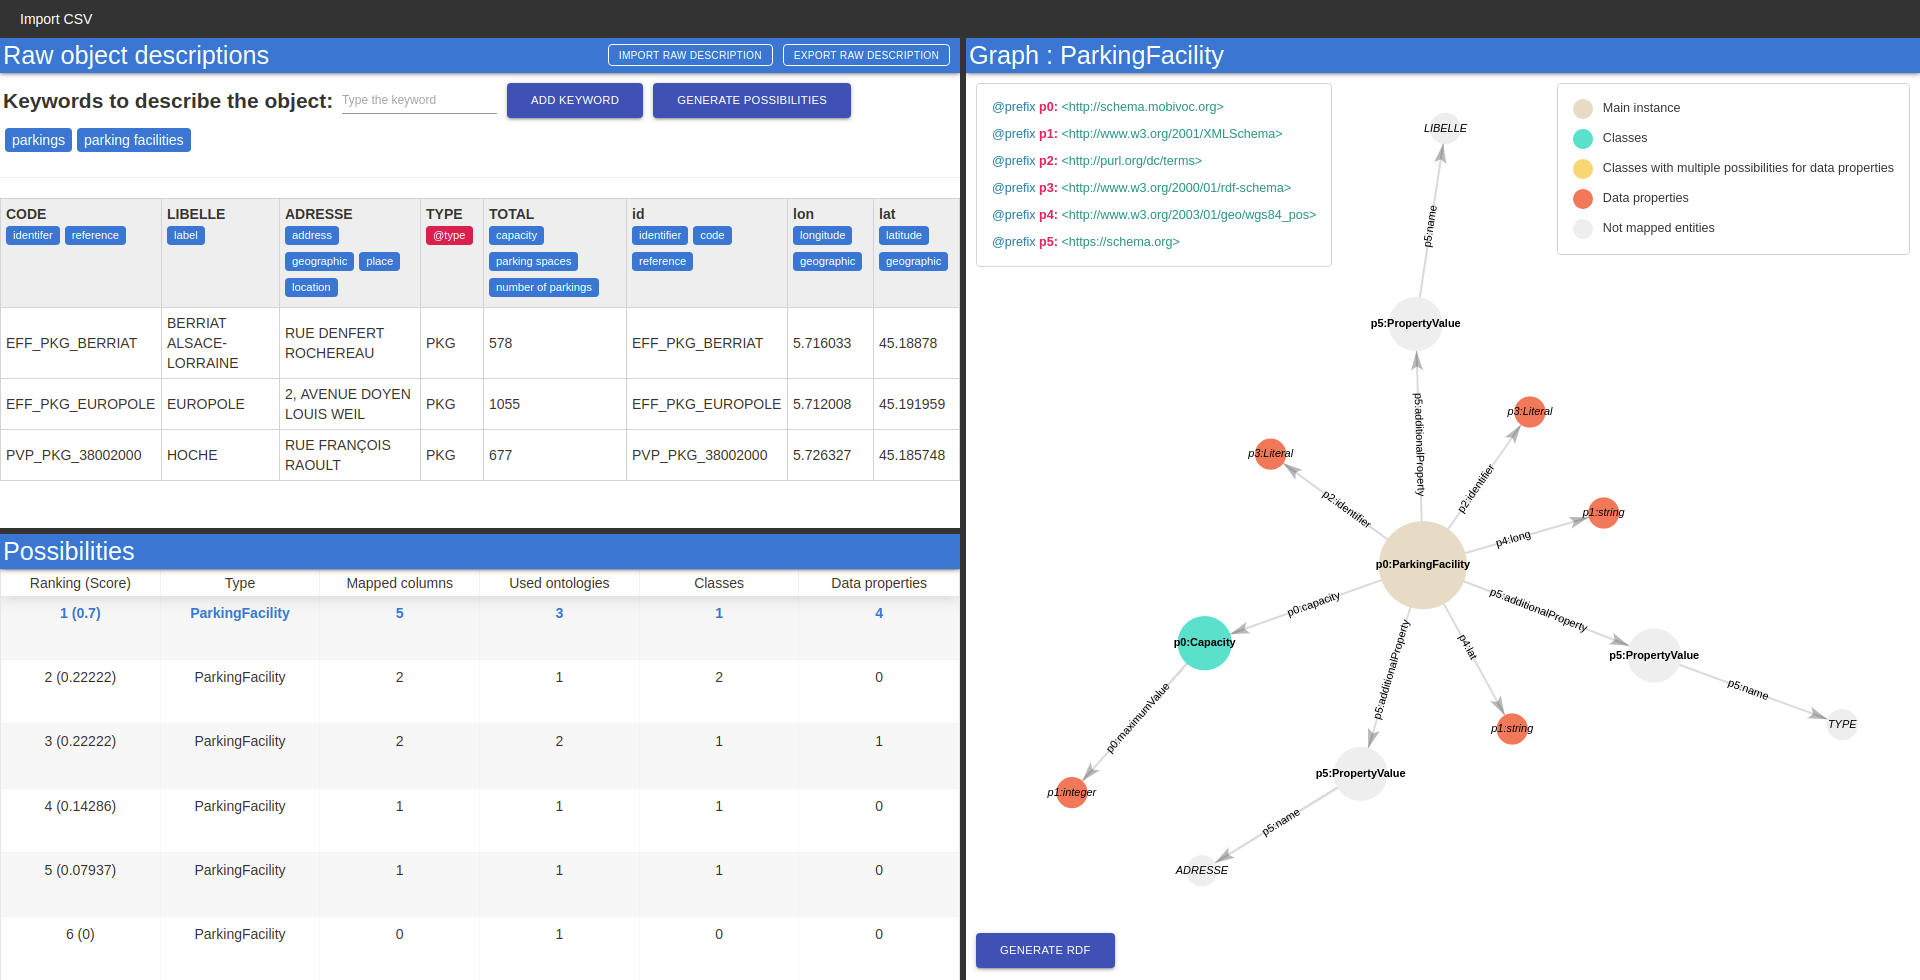
\includegraphics[scale=0.15]{images/global.png}
	\caption{Screenshot of user interface}
	\label{fig:screenshotInterface}
	\end{figure}
\end{comment}

\section{Demonstration}\label{sec:demonstration}
Our demonstration consist of using datasets from open data portals for some cities in France. \figref{expMappingParking} shows some of our experiments using these datasets. For each city, we performed two experiment. In \kword{NK}, no keywords are added by the user while in \kword{WK}, keywords are added. As we can see, even without keywords, there are fields that can be correctly mapped. Obviously, with keywords, initial mappings with better quality are generated. For all these datasets, we have their respective schema descriptions that we intend to use in our demonstration. 



\begin{figure}
	\centering
	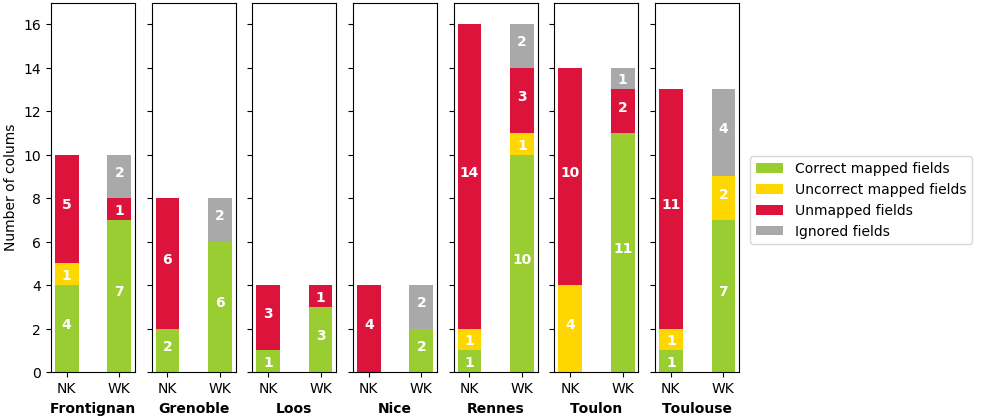
\includegraphics[scale=0.3]{./images/mappingPerParking1.png}
	\caption{Mappings of the columns grouped per parking dataset. Where \emph{NK} represents the 
		experiment without keywords and \emph{WK} represents the experiments with keywords.}
	\label{fig:expMappingParking}
\end{figure}






